%!TEX TS-program = xelatex
%!TEX options = -aux-directory=Debug -shell-escape -file-line-error -interaction=nonstopmode -halt-on-error -synctex=1 "%DOC%"
\documentclass{article}
\input{LaTeX-Submodule/template.tex}

% Additional packages & macros
\usepackage{accsupp} % PDF accessibility options
\usepackage[os=mac]{menukeys} % Format menu sequences, paths and keystrokes

\usepackage{fontawesome5}

\usepackage{tikz-uml}

%% Prevent user from selecting numbers when selecting code
\newcommand\emptyaccsupp[1]{\BeginAccSupp{ActualText={}}#1\EndAccSupp{}}

%% Custom prompt for listings environment
%%% https://tex.stackexchange.com/a/42056/224487

%%% Save the original way of printing the number
\let\othelstnumber=\thelstnumber
\def\customlinemarker#1#2{
    \edef\thelstnumber{%
        \unexpanded{%
            \ifnum#1=\value{lstnumber}\relax
              #2%
            \fi}%
        \ifx\thelstnumber\relax\else
        \expandafter\unexpanded\expandafter{\thelstnumber}%
        \fi
    }
}

% Header and footer
\newcommand{\unitName}{Programming Principles}
\newcommand{\unitTime}{Semester 1, 2022}
\newcommand{\unitCoordinator}{Dr Alan Woodley}
\newcommand{\documentAuthors}{\textsc{Tarang Janawalkar}}

\fancyhead[L]{\unitName}
\fancyhead[R]{\leftmark}
\fancyfoot[C]{\thepage}

% Copyright
\usepackage[
    type={CC},
    modifier={by-nc-sa},
    version={4.0},
    imagewidth={5em},
    hyphenation={raggedright}
]{doclicense}

\date{}

\begin{document}
%
\begin{titlepage}
    \vspace*{\fill}
    \begin{center}
        \LARGE{\textbf{\unitName}} \\[0.1in]
        \normalsize{\unitTime} \\[0.2in]
        \normalsize\textit{\unitCoordinator} \\[0.2in]
        \documentAuthors
    \end{center}
    \vspace*{\fill}
    \doclicenseThis
    \thispagestyle{empty}
\end{titlepage}
\newpage
%
\tableofcontents
\newpage
%
\lstset{language=[Sharp]C}
\lstset{morekeywords={with,is,as}}
\lstset{numbers=left, firstnumber=1, numberstyle=\ttfamily\emptyaccsupp}
\section{Programming}
\begin{definition}
    Programming is the process of designing and building an executable
    computer program to accomplish a specific computing result or to
    perform a specific task.
\end{definition}
Programming involves:
\begin{enumerate}
    \item Analysis
    \item Design
    \item Implementation
    \item Testing
\end{enumerate}
\subsection{Analysis}
Identify
\begin{itemize}
    \item the problem
    \item data, input, and output
    \item relationships between inputs and outputs
    \item constraints
\end{itemize}
\subsection{Design}
\begin{itemize}
    \item Specify modules required to implement the solution
    \item Determine how modules will integrate with the system and other modules
    \item Create tests for individual modules
    \item Create tests for the complete system
\end{itemize}
\subsection{Implementation}
\begin{itemize}
    \item Select suitable algorithms and data structures for design
    \item Write code to implement the algorithms and data structures
\end{itemize}
\subsection{Testing}
\begin{itemize}
    \item Before writing code, create a testing environment to validate the program
\end{itemize}
\section{Types and Expressions}
\subsection{Expressions}
\begin{definition}[Expressions]
    An expression is a combination of values, variables, and operators.
    In interactive mode, an interpreter evaluates expressions and displays the result.
    However, in a script, we must first compile the program to an executable in order
    to perform any tasks.
\end{definition}
\begin{definition}[Type]
    The type of an expression is ``what kind of data'' the expression carries.
\end{definition}
\begin{definition}[Variables]
    Variables are a kind of expression which have an \textbf{identity} and a \textbf{value}.

    The \textbf{value} of a variable may change as a program runs, however in
    a statically typed language, the \textbf{type} of each variable is
    specified before it can be used, and \underline{never changes}.

    Variables can be declared as follows
    \begin{lstlisting}[numbers=none]
TYPE IDENTIFIER;
TYPE IDENTIFIER = EXPRESSION;\end{lstlisting}
    In the first instance, we declare the type of the variable without initialisation.
    In the second instance, we declare and initialise the variable.
\end{definition}
\begin{definition}[Literal]
    The term \textit{literal} refers to the literal representation of a value.
    For example, when disambiguating between the variable \lstinline{dog}
    and the string \lstinline{"dog"} we would say the \emph{``variable dog''} % chktex 18
    vs.\ the \emph{``string literal dog''}.
\end{definition}
C\# identifiers must take the following into account
\begin{itemize}
    \item Identifiers can contain letters, digits and the underscore character (\lstinline{_})
    \item Identifiers must begin with a letter
    \item Identifiers cannot contain whitespaces
    \item Identifiers are case sensitive (``\lstinline{Foo}'' and ``\lstinline{foo}'' are different variables) % chktex 38
    \item Reserved words such as C\# keywords cannot be used as identifiers
\end{itemize}
\subsection{Types}
There are 9 integer and 3 floating-point types in C\#, each with a different size and range. The minimum and maximum
values of any type can be determined using \lstinline{TYPE.MinValue} and \linebreak \lstinline{TYPE.MaxValue}.
\begin{table}[H]
    \centering
    \begin{tabular}{c c c}
        \toprule
        \textbf{C\# type}  & \textbf{Size} & \textbf{Range}                \\
        \midrule
        \lstinline!sbyte!  & 8-bit         & \(-2^7\) to \(2^7 - 1\)       \\
        \lstinline!byte!   & 8-bit         & \(0\) to \(2^8 - 1\)          \\
        \lstinline!short!  & 16-bit        & \(-2^{15}\) to \(2^{15} - 1\) \\
        \lstinline!ushort! & 16-bit        & \(0\) to \(2^{16} - 1\)       \\
        \lstinline!int!    & 32-bit        & \(-2^{31}\) to \(2^{31} - 1\) \\
        \lstinline!uint!   & 32-bit        & \(0\) to \(2^{32} - 1\)       \\
        \lstinline!long!   & 64-bit        & \(-2^{63}\) to \(2^{63} - 1\) \\
        \lstinline!ulong!  & 64-bit        & \(0\) to \(2^{64} - 1\)       \\
        \bottomrule
    \end{tabular}
    \caption{Integer types in C\#.}
    % \label{}
\end{table}
\begin{table}[H]
    \centering
    \begin{tabular}{c c c c}
        \toprule
        \textbf{C\# type}   & \textbf{Size} & \textbf{Range}                                              & \textbf{Precision}   \\
        \midrule
        \lstinline!float!   & 32-bit        & \(\pm 1.5 \times 10^{-45}\) to \(\pm 3.4 \times 10^{38}\)   & \sim 6 to 9 digits   \\
        \lstinline!double!  & 64-bit        & \(\pm 5.0 \times 10^{-324}\) to \(\pm 1.7 \times 10^{308}\) & \sim 15 to 17 digits \\
        \lstinline!decimal! & 128-bit       & \(\pm 1.0 \times 10^{-28}\) to \(7.9228 \times 10^{28}\)    & \sim 28 to 29 digits \\
        \bottomrule
    \end{tabular}
    \caption{Floating-point types in C\#.}
    % \label{}
\end{table}
\subsection{Type Conversion}
By default, C\# automatically assigns the \lstinline{int}, \lstinline{uint},
\lstinline{long}, or \lstinline{ulong} type to any integer \linebreak depending the size and sign
of the provided number. Any floating-point number is instantiated as a \lstinline{double}.
\begingroup
\let\thelstnumber\relax
\customlinemarker{1}{\$}
\customlinemarker{3}{\$}
\customlinemarker{5}{\$}
\customlinemarker{7}{\$}
\begin{lstlisting}
(100).GetType()
[System.Int32]
(4294967295).GetType()    
[System.UInt32]
(-4294967295).GetType()
[System.Int64]
(100.0).GetType()
[System.Double]
\end{lstlisting}
\endgroup
To override this behaviour we can add a suffix to the number.
\begin{table}[H]
    \centering
    \begin{tabular}{c c}
        \toprule
        \textbf{Type}       & \textbf{Suffix}                                \\
        \midrule
        \lstinline!uint!    & \lstinline!u!                                  \\
        \lstinline!long!    & \lstinline!l!                                  \\
        \lstinline!ulong!   & \lstinline!u!, \lstinline!l! or \lstinline!ul! \\
        \midrule
        \lstinline!float!   & \lstinline!f!                                  \\
        \lstinline!double!  & \lstinline!d!                                  \\
        \lstinline!decimal! & \lstinline!m!                                  \\
        \bottomrule
    \end{tabular}
    \caption{Type suffixes for numeric types.}
    % \label{}
\end{table}
If a literal is prefixed with \lstinline{u}, its type is the first
of the following types in which its value can be represented:
\lstinline{uint}, \lstinline{ulong}.

Similarly, if a literal is prefixed with \lstinline{l}, its type is the first
of the following types in which its value can be represented:
\lstinline{long}, \lstinline{ulong}.

If the value of an integer is within the range of the destination type,
the value can be implicitly converted to the remaining integer types.
\subsubsection{Implicit Conversion}
Implicit conversions do not require special syntax as the conversion
always succeeds and no data is lost.

The following diagram illustrates all possible implicit conversions for numeric types
where the direction of the arrow indicates possible implicit conversions where
intermediate types can be skipped.

Note that all integer types can be converted to floating-point types.
\begin{figure}[H]
    \centering
    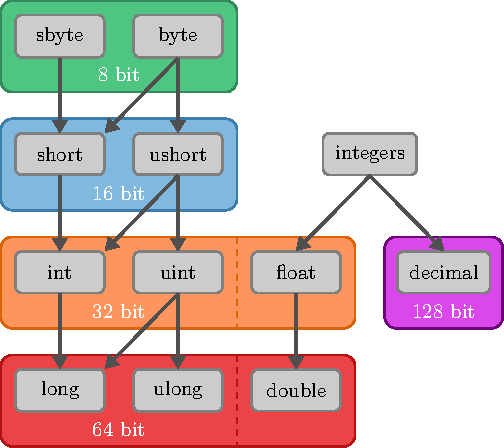
\includegraphics[height = 8cm, keepaspectratio = true]{figures/implicit_conversions.pdf}
    \caption{Numeric type implicit conversions in C\#.}
    % \label{}
\end{figure}
For example
\begingroup
\let\thelstnumber\relax
\customlinemarker{1}{\$}
\customlinemarker{2}{\$}
\customlinemarker{4}{\$}
\customlinemarker{7}{\$}
\customlinemarker{8}{\$}
\customlinemarker{10}{\$}
\begin{lstlisting}
// 8-bit unsigned integer to 64-bit signed integer 
byte b = 32; Console.WriteLine($"{b} {b.GetType()}")
32 System.Byte
long l = b; Console.WriteLine($"{l} {l.GetType()}")
32 System.Int64

// 16-bit signed integer to double precision floating-point number
short s = 30000; Console.WriteLine($"{s} {s.GetType()}")
30000 System.Int16
double d = s; Console.WriteLine($"{d} {d.GetType()}")
30000 System.Double
\end{lstlisting}
\endgroup
\subsubsection{Explicit Conversion}
When a conversion cannot be made without risking losing information,
the compiler requires that we perform an explicit conversion using a \textbf{type cast}.
The syntax for a type cast is as follows
\begin{lstlisting}[numbers=none]
(NEW_TYPE) EXPRESSION
\end{lstlisting}
For example
\begingroup
\let\thelstnumber\relax
\customlinemarker{1}{\$}
\customlinemarker{2}{\$}
\customlinemarker{4}{\$}
\customlinemarker{7}{\$}
\customlinemarker{8}{\$}
\customlinemarker{10}{\$}
\begin{lstlisting}
// Decimal to single precision floating-point number
decimal pi = 3.14159265358979323m; Console.WriteLine($"{pi} {pi.GetType()}")
3.14159265358979323 System.Decimal
float fPi = (float) pi; Console.WriteLine($"{fPi} {fPi.GetType()}")
3.141593 System.Single

// 32-bit unsigned integer to 8-bit signed integer
uint u = 9876; Console.WriteLine($"{u} {u.GetType()}")
9876 System.UInt32
byte b = (byte) u; Console.WriteLine($"{b} {b.GetType()}")
148 System.Byte
\end{lstlisting}
\endgroup
In the final example, to understand what is happening in the explicit conversion,
we must look at the binary representation of the two integers.
\begingroup
\let\thelstnumber\relax
\customlinemarker{1}{\$}
\customlinemarker{3}{\$}
\begin{lstlisting}
uint u = 9876; Console.WriteLine(Convert.ToString(u, 2).PadLeft(32, '0'))
00000000000000000010011010010100
byte b = (byte) u; Console.WriteLine(Convert.ToString(b, 2).PadLeft(8, '0'))
10010100
\end{lstlisting}
\endgroup
Notice that the value is determined by copying the 8 least significant bits
from the 32-bit unsigned integer.
\subsection{Operators}
The following table lists the C\# operators starting with the highest precedence to the lowest.
\begin{table}[H]
    \centering
    \begin{tabular}{>{\centering}p{0.45\linewidth} c}
        \toprule
        \textbf{Operators}                                                                                           & \textbf{Category}                 \\
        \midrule
        \lstinline!x.y!, \lstinline!f(x)!, \lstinline!a[i]!, \lstinline!x++!,
        \lstinline!x--!, \lstinline?x!?, \lstinline!x->y! and other keywords                                         & Primary                           \\
        \lstinline!+x!, \lstinline!-x!, \lstinline?!x?, \lstinline!~x!,
        \lstinline!++x!, \lstinline!--x!, \lstinline!^x!, \lstinline!(T)x!, \lstinline!await!,
        \lstinline!&x!, \lstinline!*x!, \lstinline!true!, \lstinline!false!                                          & Unary                             \\
        \lstinline!x..y!                                                                                             & Range                             \\
        \lstinline!switch!, \lstinline!with!                                                                         & ---                               \\
        \lstinline!x * y!, \lstinline!x / y!, \lstinline!x % y!                                                      & Multiplicative                    \\
        \lstinline!x + y!, \lstinline!x - y!                                                                         & Additive                          \\ % chktex 8
        \lstinline!x << y!, \lstinline!x >> y!                                                                       & Shift                             \\
        \lstinline!x < y!, \lstinline!x > y!, \lstinline!x <= y!, \lstinline!x >= y!, \lstinline!is!, \lstinline!as! & Relational and type-testing       \\
        \lstinline!x == y!, \lstinline?x != y?                                                                       & Equality                          \\ % chktex 26
        \lstinline!x & y!                                                                                            & Logical {\ttfamily{AND}}          \\
        \lstinline!x ^ y!                                                                                            & Logical {\ttfamily{XOR}}          \\
        \lstinline!x | y!                                                                                            & Logical {\ttfamily{OR}}           \\
        \lstinline!x && y!                                                                                           & Conditional {\ttfamily{AND}}      \\
        \lstinline!x || y!                                                                                           & Conditional {\ttfamily{OR}}       \\
        \lstinline!x ?? y!                                                                                           & Null-coalescing operator          \\ % chktex 26
        \lstinline!c ? t : f!                                                                                        & Conditional operator              \\ % chktex 26
        \lstinline!x = y!, \lstinline!=>! and shorthand assignments                                                  & Assignment and lambda declaration \\
        \bottomrule
    \end{tabular}
    \caption{Precedence of various operators in C\#.}
    % \label{}
\end{table}
In C\#, arithmetic operations behave as expected.
\begingroup
\let\thelstnumber\relax
\customlinemarker{1}{\$}
\customlinemarker{3}{\$}
\customlinemarker{5}{\$}
\customlinemarker{7}{\$}
\customlinemarker{9}{\$}
\begin{lstlisting}
123 + 12
135
123 - 12
111
123 * 12
1476
123 / 12
10
123 % 12
3
\end{lstlisting}
\endgroup
All results in the example above are of type \lstinline{System.Int32}.

Binary operators always convert the resulting data type to the data type of the
argument with the largest size in memory
(with a few exceptions when converting between floating-point types).

Hence division between two 32-bit integers truncates any floating-point precision.
\begingroup
\let\thelstnumber\relax
\customlinemarker{1}{\$}
\customlinemarker{3}{\$}
\customlinemarker{5}{\$}
\customlinemarker{7}{\$}
\begin{lstlisting}
123 / 12
10
123.0 / 12
10.25
123 / 12.0
10.25
123.0 / 12.0
10.25
\end{lstlisting}
\endgroup
Here only the latter three expressions are converted to \lstinline{System.Double}.
\subsection{Characters}
A character type represents a \textbf{single} Unicode UTF-16 character.
Character objects can be implicitly converted to 16-bit unsigned integers and
support the comparison, equality, increment and decrement operators.

A character is initialised using single quotation marks (\lstinline{'}). % chktex 38
\begingroup
\let\thelstnumber\relax
\customlinemarker{1}{\$}
\customlinemarker{3}{\$}
\customlinemarker{5}{\$}
\customlinemarker{7}{\$}
\customlinemarker{9}{\$}
\begin{lstlisting}
char c = 'A'; c
'A'
c.GetType()
[System.Char]
c++
'B'
(ushort) c
69
c == 69
true
\end{lstlisting}
\endgroup
\subsection{Strings}
A string is a sequential read-only collection of character objects that
is initialised using double quotation marks (\lstinline{"}). % chktex 18
\begingroup
\let\thelstnumber\relax
\customlinemarker{1}{\$}
\customlinemarker{3}{\$}
\begin{lstlisting}
string s = "Hello, World!"; s
"Hello, World!"
s.GetType()
[System.String]
\end{lstlisting}
\endgroup
\subsubsection{String Indexing}
The characters in a string can be accessed by position using indexing (starting at 0).
\begingroup
\let\thelstnumber\relax
\customlinemarker{1}{\$}
\customlinemarker{3}{\$}
\begin{lstlisting}
s[0]
'H'
s[s.Length - 1]
'!'
\end{lstlisting}
\endgroup
\subsubsection{Immutability}
In C\#, string objects are immutable meaning that the string cannot be modified in memory. If a new string is assigned
to this object, it will simply point to a new location in memory.
\begingroup
\let\thelstnumber\relax
\customlinemarker{1}{\$}
\customlinemarker{3}{\$}
\customlinemarker{6}{\$}
\begin{lstlisting}
string s = "String with tyop."; s
"String with tyop."
s[14] = 'p';
(1,1): error CS0200: Property or indexer 'string.this[int]' cannot be assigned 
to -- it is read only
s = "String without typo."
"String without typo."
\end{lstlisting}
\endgroup
\subsubsection{Escape Sequences}
To use special characters such as newlines, tabs, backslashes, or double quotation marks, we must
use an escape sequence.
\begingroup
\let\thelstnumber\relax
\customlinemarker{1}{\$}
\begin{lstlisting}
string s = "This is a quotation mark \".\nThis line appears on a new line."; s
"This is a quotation mark \".\nThis line appears on a new line."
\end{lstlisting}
\endgroup
Note that the string is evaluated as a string literal. To view this string verbatim, we must use
\lstinline{Console.WriteLine}.
\begingroup
\let\thelstnumber\relax
\customlinemarker{1}{\$}
\begin{lstlisting}
Console.WriteLine(s) 
This is a quotation mark ".
This line appears on a new line.
\end{lstlisting}
\endgroup
\subsubsection{Verbatim String Literals}
If a string contains many escape sequences we can use verbatim strings for convenience.
\begingroup
\let\thelstnumber\relax
\customlinemarker{1}{\$}
\customlinemarker{3}{\$}
\begin{lstlisting}
string s = @"String with multiple escape sequences ""This is a quote"".
This line appears on a new line.";
Console.WriteLine(s)
String with multiple escape sequences "This is a quote".
This line appears on a new line.
\end{lstlisting}
\endgroup
\subsubsection{Format Strings}
To dynamically determine a string at runtime, we can use format strings.
There are two methods to create format strings: string interpolation and composite formatting.

String interpolation allows us to reference variable names directly inside a string.
Interpolated strings are identified by the dollar sign.
\begingroup
\let\thelstnumber\relax
\customlinemarker{1}{\$}
\customlinemarker{2}{\$}
\begin{lstlisting}
int a = 40; int b = 13;
$"Given a = {a} and b = {b}, a + b = {a + b}"
"Given a = 40 and b = 13, a + b = 53"
\end{lstlisting}
\endgroup
Composite formatting uses placeholders for variables which must be provided in order of reference.
Here the same variable can be referenced many times in a string.
\begingroup
\let\thelstnumber\relax
\customlinemarker{1}{\$}
\customlinemarker{2}{\$}
\customlinemarker{4}{\$}
\customlinemarker{6}{\$}
\begin{lstlisting}
int a = 40; int b = 13;
string.Format("Given a = {0} and b = {1}, a + b = {2}", a, b, a + b)
"Given a = 40 and b = 13, a + b = 53"
string.Format("a + b = {2} where a = {0} and b = {1}", a, b, a + b)
"a + b = 53 where a = 40 and b = 13"
string.Format("We can reference `a` twice, here {0} and here {0}", a)
"We can reference `a` twice, here 40 and here 40"
\end{lstlisting}
\endgroup
\subsubsection{Numeric to String Conversion}
Strings can be concatenated with numeric variables
\begingroup
\let\thelstnumber\relax
\customlinemarker{1}{\$}
\customlinemarker{2}{\$}
\begin{lstlisting}
int a = 25;
"The temperature is " + a + " degrees."
"The temperature is 25 degrees."
\end{lstlisting}
\endgroup
As the \lstinline{+} operator is evaluated from left to right, the following string concatenation
will not evaluate the sum of 1, 2, and 3.
\begingroup
\let\thelstnumber\relax
\customlinemarker{1}{\$}
\begin{lstlisting}
"sum = " + 1 + 2 + 3
"sum = 123"
\end{lstlisting}
\endgroup
The \lstinline{ToString()} method can be accessed from all numeric types, with a
format specifier which indicates the number of precision to display.
\begingroup
\let\thelstnumber\relax
\customlinemarker{1}{\$}
\customlinemarker{3}{\$}
\customlinemarker{5}{\$}
\begin{lstlisting}
(1498).ToString("G3")
"1.5E+03"
(1498).ToString("F3")
"1498.000"
(1498).ToString("C2")
"$1,498.00"
\end{lstlisting}
\endgroup
These format specifiers can be applied directly in interpolated strings.
\begingroup
\let\thelstnumber\relax
\customlinemarker{1}{\$}
\customlinemarker{2}{\$}
\begin{lstlisting}
int i = 1498;
$"{i:G3}, {i:F3}, {i:C2}"
"1.5E+03, 1498.000, $1,498.00"
\end{lstlisting}
\endgroup
We can also add specify padding in interpolated strings.
\begingroup
\let\thelstnumber\relax
\customlinemarker{1}{\$}
\customlinemarker{2}{\$}
\begin{lstlisting}
decimal pi = 3.14159265358979323m;
$"Pi with left padding {pi, 10:F6}"
"Pi with left padding   3.141593"
\end{lstlisting}
\endgroup
For more information see: \href{https://docs.microsoft.com/en-us/dotnet/standard/base-types/custom-numeric-format-strings}{\textit{Custom numeric format strings}}.
\subsubsection{String to Numeric Conversion}
We can convert a string to a number by calling the \lstinline{Parse} method found on numeric types,
or by using methods in the \lstinline{System.Convert} class.
\begingroup
\let\thelstnumber\relax
\customlinemarker{1}{\$}
\customlinemarker{3}{\$}
\begin{lstlisting}
double.Parse("2.718281")
2.718281
Convert.ToDouble("2.718281")
2.718281
\end{lstlisting}
\endgroup
\section{Structured Programming}
Structured programming relies on three constructs: sequence, selection and iteration.
These help us control the flow of our programs.
\subsection{Sequence}
\subsubsection{Blocks}
In C\# we can group statements together inside a scope by using braces \lstinline!{ }!.
The statements inside this block are executed in order as a single instruction.
\begingroup
\let\thelstnumber\relax
\customlinemarker{1}{\$}
\customlinemarker{2}{.}
\customlinemarker{3}{.}
\customlinemarker{4}{.}
\customlinemarker{5}{.}
\customlinemarker{7}{\$}
\begin{lstlisting}
int i = 5;
{
    i = 10;
    Console.WriteLine(i);
}
10
Console.WriteLine(i);
10
\end{lstlisting}
\endgroup
Here \lstinline{i} is accessed as an enclosing locally scoped variable.
\emph{This behaviour is akin to blocks defined in selection and iteration structures.}
\subsubsection{Nested Blocks}
Here is another example that utilises nested blocks and demonstrates access.

\begingroup
\let\thelstnumber\relax
\customlinemarker{1}{\$}
\customlinemarker{2}{\$}
\customlinemarker{3}{.}
\customlinemarker{4}{.}
\customlinemarker{5}{.}
\customlinemarker{6}{.}
\customlinemarker{7}{.}
\customlinemarker{8}{.}
\customlinemarker{9}{.}
\customlinemarker{10}{.}
\customlinemarker{11}{.}
\customlinemarker{12}{.}
\customlinemarker{13}{\$}
\begin{lstlisting}
// Global scope    
{
    // Block 1     
    int i = 5;  
    Console.WriteLine(i);
    {
        // Block 2
        i += 5;
        Console.WriteLine(i);
    }
    // i = 10
}
Console.WriteLine(i);
5
10
(1,19): error CS0103: The name 'i' does not exist in the current context
\end{lstlisting}
\endgroup
In this example, we see that the variable \lstinline{i} is local to block 1 and therefore accessible to block 2.

However, the converse is not true. \lstinline{i} cannot be accessed by its enclosing scope
as local variables are destroyed when a block ends.

We also cannot declare a variable in a block that shares its name
with another variable in its enclosing local scope.
\begingroup
\let\thelstnumber\relax
\customlinemarker{1}{\$}
\customlinemarker{2}{.}
\customlinemarker{3}{.}
\customlinemarker{4}{.}
\customlinemarker{5}{.}
\customlinemarker{6}{.}
\begin{lstlisting}
{
    int i = 5;
    {
        int i = 5;
    }   
}
(4,13): error CS0136: A local or parameter named 'i' cannot be declared
in this scope because that name is used in an enclosing local scope to 
define a local or parameter
\end{lstlisting}
\endgroup
\subsection{Selection}
Selection allows us to choose from a range of different options.
\subsubsection{If Statements}
If statements have the following syntax.
\begin{lstlisting}[numbers=none]
// Single statement
if (CONDITION) STATEMENT;
// Multiple statements
if (CONDITION)
{
    STATEMENTS
}
\end{lstlisting}
In both cases, \lstinline{CONDITION} is an expression that returns a Boolean value % chktex 13
when evaluated. If this value is \lstinline{true}, the subsequent statement(s) will
be executed. Conversely, if the expression yields \lstinline{false}, the subsequent
statement(s) will be ignored and control passes to the next statement after the \lstinline{if}
statement.
\subsubsection{If-else Statements}
We can add an alternative statement if \lstinline{CONDITION} is \lstinline{false} using an \lstinline{else} % chktex 13
clause.
\begin{lstlisting}[numbers=none]
// Single statement
if (CONDITION) STATEMENT_1 else STATEMENT_2;
// Multiple statements
if (CONDITION) 
{
    STATEMENTS_1
} else
{
    STATEMENTS_2;
}
\end{lstlisting}
This structure differs from the previous example as either \lstinline{STATEMENT_1} or \lstinline{STATEMENT_2}
can be executed. This decision depends on the Boolean value returned by the condition.
\subsubsection{Nested if Statements}
The blocks in an \lstinline{if} statement also allow us to nest any number of
\lstinline{if} statements to create a complex flow of control.
\begin{lstlisting}[numbers=none]
if (CONDITION_1) if (CONDITION_2) STATEMENT_2 else STATEMENT_1;
// Written using braces
if (CONDITION_1) 
{
    if (CONDITION_2) 
    {
        STATEMENT_2
    }
} else 
{
    STATEMENT_1
}
\end{lstlisting}
Generally, nested \lstinline{if} statements are difficult to read and should be avoided if possible.
\subsubsection{Cascading if Statements}
An alternative to nested \lstinline{if} statements are cascading \lstinline{if} statements.
These statements allow us to provide controlled alternatives to an \lstinline{if-else} statement if the
first condition returns \lstinline{false}.
\begin{lstlisting}[numbers=none]
if (CONDITION_1) 
{
    STATEMENTS_1
} else if (CONDITION_2)
{
    STATEMENTS_2
} else if (CONDITION_3)
{
    STATEMENTS_3
} 
...
else {
    STATEMENTS_N
}
\end{lstlisting}
In this structure, any statement \(1<i<n\) will be executed if
and only if all conditions before \(i\) yield \lstinline{false} and
\lstinline{CONDITION_I} yields \lstinline{true}. % chktex 13

The final statement \(n\) after the \lstinline{else} clause is executed
if all preceding conditions return \lstinline{false}.

Note that the \lstinline{else} clause may be omitted.
\subsubsection{Switch Statements}
A \lstinline{switch} statement is an alternative to cascading \lstinline{if}
statements and are another kind of multi-way branch.
\begin{lstlisting}[numbers=none]
switch (EXPRESSION) 
{
    case CONSTANT_1:
        STATEMENTS_1;
        break;
    case CONSTANT_2:
        STATEMENTS_2;
        break;
    ...
    default:
        STATEMENTS_N;
        break;
}
\end{lstlisting}
In this structure, \lstinline{EXPRESSION} is any numeric or string expression, % chktex 13
and \lstinline{CONSTANT} is a literal of matching type. % chktex 13
This means that \lstinline{STATEMENTS_I} is executed if \lstinline{EXPRESSION == CONSTANT_I}. % chktex 13

The default branch behaves similarly to an \lstinline{else} clause and it is executed if
none of the preceding cases are satisfied.

Each branch must end with one of the following keywords depending on where the
switch statement is defined: \lstinline{break}, \lstinline{return},
\lstinline{goto}, \lstinline{throw}, or \lstinline{continue}.
\subsection{Iteration}
Iterative constructs allow us to repeat statements zero, one, or many times,
without making multiple copies of the statement.
\subsubsection{While Statements}
\begin{lstlisting}[numbers=none]
while (CONDITION) 
{
    STATEMENTS
}
\end{lstlisting}
Fundamental semantics:
\begin{enumerate}
    \item Execute \lstinline{STATEMENTS} if \lstinline{CONDITION == true}. % chktex 13
    \item Goto Step 1.
\end{enumerate}
\subsubsection{Do-while Statements}
\begin{lstlisting}[numbers=none]
do 
{
    STATEMENTS
}
while (CONDITION) 
\end{lstlisting}
Fundamental semantics:
\begin{enumerate}
    \item Execute \lstinline{STATEMENTS}. % chktex 13
    \item Goto Step 1 if \lstinline{CONDITION == true}.
\end{enumerate}
\subsubsection{For Statements}
\begin{lstlisting}[numbers=none]
for (INIT; CONDITION; UPDATE) 
{
    STATEMENTS
}
\end{lstlisting}
Fundamental semantics:
\begin{enumerate}
    \item Execute \lstinline{INIT}. % chktex 13
    \item Execute \lstinline{STATEMENTS} if \lstinline{CONDITION == true}. % chktex 13
    \item Execute \lstinline{UPDATE}.
    \item Goto Step 2.
\end{enumerate}
Generally, a \lstinline{while} statement is used when the number of iterations is unknown and
\lstinline{for} statements are used otherwise. Both of these structures can execute
statements either zero, one or many times.

While uncommon, \lstinline{do-while} statements are used if we want to execute
the loop body at least once.
\subsection{Jump Statements}
The following statements unconditionally transfer control:
\begin{itemize}
    \item \lstinline{break} terminates the closest enclosing iteration or switch statement
    \item \lstinline{continue} starts a new iteration of the closest enclosing iteration statement
\end{itemize}
Note that jump statements can be placed anywhere inside the loop body and that any succeeding
statements or the \lstinline{UPDATE} statement (in the \lstinline{for} structure) % chktex 13
will not be executed.
\subsection{Booleans}
A Boolean (\lstinline{bool}) is a type that has two values,
\lstinline{true} and \lstinline{false}.
Boolean expressions are expressions that when evaluated, yield a Boolean value.
\subsubsection{Comparison Operators}
Comparison operators are a common Boolean expression:
\begin{itemize}
    \item \lstinline{x == y}
    \item \lstinline+x != y+ % chktex 26
    \item \lstinline{x < y}
    \item \lstinline{x > y}
    \item \lstinline{x <= y}
    \item \lstinline{x >= y}
\end{itemize}
\subsubsection{Logical Operators}
Logical operators are also Boolean expressions:
\begin{itemize}
    \item \lstinline+!a+ (not)
    \item \lstinline{a && b} (and)
    \item \lstinline{a || b} (or)
\end{itemize}
In C\#, logical operators use short-circuit evaluation, meaning that
if the left expression guarantees the resulting Boolean value,
the right expression is not evaluated.

For example
\begingroup
\let\thelstnumber\relax
\customlinemarker{1}{\$}
\customlinemarker{2}{.}
\customlinemarker{3}{.}
\customlinemarker{4}{.}
\customlinemarker{5}{.}
\customlinemarker{6}{\$}
\customlinemarker{7}{.}
\customlinemarker{8}{.}
\customlinemarker{9}{.}
\customlinemarker{10}{.}
\customlinemarker{11}{\$}
\begin{lstlisting}
bool a() 
{ 
    Console.WriteLine("a was executed."); 
    return false;
}
bool b() 
{ 
    Console.WriteLine("b was executed."); 
    return true;
}
a() && b()
a was executed.
False
\end{lstlisting}
\endgroup
Here we see that the second function \lstinline{b()} was not executed
as the {\ttfamily AND} operator requires both expressions to be true,
so regardless of the value of \lstinline{b()}, the result will be
\lstinline{false}.

Similarly for {\ttfamily OR}:
\begingroup
\let\thelstnumber\relax
\customlinemarker{1}{\$}
\customlinemarker{2}{.}
\customlinemarker{3}{.}
\customlinemarker{4}{.}
\customlinemarker{5}{.}
\customlinemarker{6}{\$}
\customlinemarker{7}{.}
\customlinemarker{8}{.}
\customlinemarker{9}{.}
\customlinemarker{10}{.}
\customlinemarker{11}{\$}
\begin{lstlisting}
bool a() 
{ 
    Console.WriteLine("a was executed."); 
    return false;
}
bool b() 
{ 
    Console.WriteLine("b was executed."); 
    return true;
}
b() || a()
b was executed.
True
\end{lstlisting}
\endgroup
Here only one of the two expressions needs to evaluate to \lstinline{true}
for the result to be true. However, if we reversed the order of
the expressions:
\begingroup
\let\thelstnumber\relax
\customlinemarker{1}{\$}
\customlinemarker{2}{.}
\customlinemarker{3}{.}
\customlinemarker{4}{.}
\customlinemarker{5}{.}
\customlinemarker{6}{\$}
\customlinemarker{7}{.}
\customlinemarker{8}{.}
\customlinemarker{9}{.}
\customlinemarker{10}{.}
\customlinemarker{11}{\$}
\begin{lstlisting}
bool a() 
{ 
    Console.WriteLine("a was executed."); 
    return false;
}
bool b() 
{ 
    Console.WriteLine("b was executed."); 
    return true;
}
a() || b()
a was executed.
b was executed.
True
\end{lstlisting}
\endgroup
we can see that since \lstinline{a()} does not guarantee
the resulting Boolean value, we must also evaluate \lstinline{b()}.

The {\ttfamily NOT} operator simply negates the value of the Boolean expression.
\section{Collections}
\subsection{Arrays}
If we want to effectively manage groups of related objects, we can utilise arrays and collections.
When defining an array of type \lstinline{T}, we must append the type with square brackets \lstinline{[ ]}.
\begin{lstlisting}[numbers=none]
TYPE[] IDENTIFIER;
TYPE[] IDENTIFIER = EXPRESSION;
\end{lstlisting}
As a result, each item must have the same data type. To specify the array size, we can initialise
the variable with the \lstinline{new} expression.
\begin{lstlisting}[numbers=none]
TYPE[] IDENTIFIER = new TYPE[SIZE];
// Alternatively
TYPE[] IDENTIFIER;
IDENTIFIER = new TYPE[SIZE];
\end{lstlisting}
\subsection{Access}
To access the array, we can use the identifier for that array. Each object within
an array can be distinguished by its subscript (or index). To access the object within
an array, we place the index inside square brackets \lstinline{[i]} and append this to the
identifier.
\begingroup
\let\thelstnumber\relax
\customlinemarker{1}{\$}
\customlinemarker{2}{\$}
\customlinemarker{4}{\$}
\customlinemarker{6}{\$}
\customlinemarker{8}{\$}
\customlinemarker{10}{\$}
\begin{lstlisting}
int[] intArray = new int[3]; 
intArray
int[3] { 0, 0, 0 }
intArray[0] = 1; intArray[0]
1
intArray[1] = 2; intArray[0]
2
intArray[2] = 3; intArray[0]
3
intArray
int[3] { 1, 2, 3 }
\end{lstlisting}
\endgroup
Note that array indexing starts at 0. If the value of the elements inside the array
are known when the array is initialised, we can set the element values using the following syntax.
\begin{lstlisting}[numbers=none]
TYPE[] IDENTIFIER = new TYPE[SIZE] { element1, element2, ..., elementN };
TYPE[] IDENTIFIER = new TYPE[] { element1, element2, ..., elementN };
TYPE[] IDENTIFIER = { element1, element2, ..., elementN };
\end{lstlisting}
Note that when using the first method, the number of elements \(N\) must be equal to the specified \lstinline{SIZE}. % chktex 13
\subsection{Array Representation in Memory}
To be able to access an array by index, the elements must be stored contiguously in memory, that is,
stored one after the other. This means that each element \(i\) is \(i \times S_T\) bytes from \(i = 0\),
where \(S_T\) is the size of the array type.
\subsection{Default Values}
If an array is declared without initialisation, then each element takes one of the following
default values based on the type:
\begin{description}
    \item[Numeric] \lstinline{0}
    \item[Character] \lstinline{\u0000} or \lstinline{null}
    \item[Boolean] \lstinline{false}
\end{description}
\subsection{ForEach Loops}
The \lstinline{foreach} statement provides a simple, clean way to iterate through the elements of an array,
without using the element index.
\begingroup
\let\thelstnumber\relax
\customlinemarker{1}{\$}
\customlinemarker{2}{\$}
\customlinemarker{3}{.}
\customlinemarker{4}{.}
\customlinemarker{5}{.}
\begin{lstlisting}
int[] array = { 1, 2, 3 };
foreach (int i in array)
{
    Console.WriteLine(i);
}
1
2
3    
\end{lstlisting}
\endgroup
Note that the values \lstinline{i} are read-only, and hence this structure
does not modify the elements of an array.

If we wanted to modify these values, can we use either a \lstinline{while} or
\lstinline{for} loop. The following example increments each value of an array
using a \lstinline{for} loop.
\begingroup
\let\thelstnumber\relax
\customlinemarker{1}{\$}
\customlinemarker{2}{\$}
\customlinemarker{3}{.}
\customlinemarker{4}{.}
\customlinemarker{5}{.}
\customlinemarker{6}{\$}
\begin{lstlisting}
int[] array = { 1, 2, 3 };
for (int i = 0; i < array.Length; i++)
{
    array[i]++;
}
array
int[3] { 2, 3, 4 }
\end{lstlisting}
\endgroup
\subsection{Compound Arrays}
When we have two or more arrays of values that share
the same indices, we can implement compound arrays to
create a correspondence between those arrays.
\subsubsection{Parallel Arrays}
Parallel arrays are useful when the various arrays
hold different types of data. In this method, multiple
single dimensional arrays are created.
\begingroup
\let\thelstnumber\relax
\customlinemarker{1}{\$}
\customlinemarker{2}{\$}
\customlinemarker{3}{\$}
\customlinemarker{4}{.}
\customlinemarker{5}{.}
\customlinemarker{6}{.}
\begin{lstlisting}
string[] item = { "Shoes", "Shirt", "Pants" };
int[] price = { 100, 40, 80 };
for (int i = 0; i < item.Length; i++) 
{
    Console.WriteLine($"Item: {item[i]}\tPrice: {price[i]:C}");
}
Item: Shoes     Price: $100.00
Item: Shirt     Price: $40.00
Item: Pants     Price: $80.00
\end{lstlisting}
\endgroup
Although there are benefits to using this approach, larger data
sets with multiple columns may be better represented in a
multidimensional array.
\subsubsection{Multidimensional Arrays}
Multidimensional arrays behave similarly to regular arrays
but use different declaration and access syntax.
\begin{lstlisting}[numbers=none]
// 2D arrays
TYPE[,] IDENTIFIER = new TYPE[SIZEX, SIZEY];
// nD arrays
TYPE[,,...] IDENTIFIER = new TYPE[SIZEX, SIZEY, ...];
\end{lstlisting}
When declaring the type, it is important to specify the correct
number of commas (\lstinline{,}). The number of commas is equal to
the number of dimensions minus 1.

When instantiating the array on the right hand side of the assignment,
the length of each dimension is specified as an integer, and is separated by a comma.
Similar to single dimensional arrays, we can set the values when we declare the array.
\begingroup
\let\thelstnumber\relax
\customlinemarker{1}{\$}
\customlinemarker{2}{.}
\customlinemarker{3}{\$}
\begin{lstlisting}
int[,] array2d = {{ 2, 3 },
                  { 1, 5 }};
array2d
int[2, 2] { { 2, 3 }, { 1, 5 } }
\end{lstlisting}
\endgroup
Multidimensional arrays are commonly separated at each dimension
so that they are easier to read.

When accessing the value from a multidimensional array,
we must separate each index using a comma.
\begingroup
\let\thelstnumber\relax
\customlinemarker{1}{\$}
\customlinemarker{2}{\$}
\customlinemarker{4}{\$}
\customlinemarker{5}{.}
\customlinemarker{6}{.}
\customlinemarker{7}{.}
\customlinemarker{8}{.}
\customlinemarker{9}{.}
\customlinemarker{10}{.}
\begin{lstlisting}
int ROW = array2d.GetLength(0);
int COL = array2d.GetLength(1);

for (int i = 0; i < ROW; i++)
{
    for (int j = 0; j < COL; j++)
    {
        Console.WriteLine($"The value at ({i}, {j}) is {array2d[i, j]}");
    }
}
The value at (0, 0) is 2
The value at (0, 1) is 3
The value at (1, 0) is 1
The value at (1, 1) is 5
\end{lstlisting}
\endgroup
Here the \lstinline{GetLength()} methods are used to find the length
of both the first and second dimensions.
\subsection{Lists}
Lists allow us to have variable size arrays, meaning we can
add and remove elements during execution.
\begin{lstlisting}[numbers=none]
List<TYPE> IDENTIFIER = new List<TYPE>();
List<TYPE> IDENTIFIER = new List<TYPE>{ elements };
\end{lstlisting}
The first syntax creates a list with 0 elements.
We can add to this list using the \lstinline{Add()} method, and
remove from it using the \lstinline{Remove()} method.
\begingroup
\let\thelstnumber\relax
\customlinemarker{1}{\$}
\customlinemarker{2}{\$}
\customlinemarker{4}{\$}
\customlinemarker{5}{\$}
\customlinemarker{6}{\$}
\customlinemarker{7}{\$}
\customlinemarker{8}{\$}
\customlinemarker{9}{\$}
\customlinemarker{10}{\$}
\begin{lstlisting}
List<int> list = new List<int>();
list
List<int>(0) { }
list.Add(3)
list.Add(1)
list.Add(4)
list.Add(5)
list.Add(1)
list.Add(5)
list
List<int>(6) { 3, 1, 4, 5, 1, 5 }
\end{lstlisting}
\endgroup
By using the \lstinline{Remove()} method, we can remove the
accidental 5 that appears at index 3.
\begingroup
\let\thelstnumber\relax
\customlinemarker{1}{\$}
\customlinemarker{3}{\$}
\customlinemarker{5}{\$}
\customlinemarker{7}{\$}
\begin{lstlisting}
list.Remove(5)
true
list
List<int>(5) { 3, 1, 4, 1, 5 }
list.Remove(7)
false
list
List<int>(5) { 3, 1, 4, 1, 5 }
\end{lstlisting}
\endgroup
From the first \lstinline{Remove()},
only the first \lstinline{5} was removed from the list.
The method also returned a Boolean value indicating that the value
\lstinline{5} existed in the list. When we try to remove the
number \lstinline{7}, the method returns \lstinline{false},
as the list does not contain a \lstinline{7}, and hence the
list remains unchanged.
\section{Methods}\label{section:methods}
\subsection{Programming Complexity}
Programming logic is usually complex as it involves modelling rules
and constraints from the real world.

When dealing with complexity, we must guarantee:
\begin{itemize}
    \item Correctness
          \begin{itemize}
              \item The software is trustworthy
              \item The software meets requirements
              \item Valid inputs always produce the required outcomes
          \end{itemize}
    \item Robustness
          \begin{itemize}
              \item The program does not crash
          \end{itemize}
    \item Efficiency
          \begin{itemize}
              \item The program completes its work quickly
              \item The program utilises efficient algorithms
              \item The program does not introduce unnecessary loops or convoluted logic
              \item The program uses existing standard libraries
          \end{itemize}
\end{itemize}
We can use methods to address this complexity by decomposing large tasks into smaller tasks.
\begin{itemize}
    \item Each sub-task handles part of the larger problem
    \item Each sub-task can be implemented separately as a method or group of methods
    \item Tests can be developed to target each method individually
\end{itemize}
As long as each sub-task is correct, robust, and efficient, the overall program will be also.
As sub-tasks are simpler than the original problem, these goals are easier to achieve.

Methods can also help eliminate duplicate code, so that code is more compact, and by
moving them into libraries, we can use them in other projects making programming
more productive.
\subsection{Declaring Methods}
A method has the following syntax
\begin{lstlisting}[numbers=none]
[ACCESS_MODIFIER] RETURN_TYPE METHOD_IDENTIFIER(PARAMETER_LIST)
{
    STATEMENTS
}    
\end{lstlisting}
\subsubsection{Access Modifiers}
Access modifiers will be discussed in a later section.
\subsubsection{Return Types}
A return type specifies what type of value is returned to the method caller.
If a method alters the state of the program and does not
necessarily require an output, is a side effect method and its return type is
\lstinline{void}.
\subsubsection{Identifiers}
The identifier is the name of the method, which can be any valid C\# identifier.
By convention, method identifiers are camel-case with an upper-case first letter.
\subsubsection{Parameter List}
The parameter list declares the formal parameters of the method, i.e.,
what arguments may be passed to the method. The parameter list is
a comma-separated list of parameters that have the following syntax
\begin{lstlisting}[numbers=none]
[PARAMETER_MODIFIER] TYPE PARAMETER_IDENTIFIER [= DEFAULT_VALUE]
\end{lstlisting}
The parameter modifier tells the compiler whether to send an argument by reference
or by value. There are 4 modifiers to choose from
\begin{itemize}
    \item \lstinline{in} --- Arguments are passed by reference but cannot be modified.
    \item \lstinline{ref} --- Arguments are passed by reference and can be modified.
    \item \lstinline{out} --- Arguments are passed by reference but must be initialised inside the method.
    \item \lstinline{params} --- A variable number of arguments are passed by value.
\end{itemize}
By default, if a modifier is not specified, the argument is generally passed by value.

The parameter type specifies what type of argument is to be passed. The parameter identifier
gives the argument an alias within the method's scope, and
default values can be assigned to parameters if they are optional.

Note that parameters do not need to be re-declared inside the method.
\subsubsection{Statements}
The statements inside a method can consist of sequences of statements
including declarations, expressions, and structured blocks.
As a method introduces a nested block, all variables declared in a method body
are local to the method.
\subsection{Invoking Methods}
To call a method we can invoke it using the following syntax
\begin{lstlisting}[numbers=none]
METHOD_IDENTIFIER(ARGUMENT_LIST)
\end{lstlisting}
If a method is defined in another class, we must qualify the name
with the appropriate class:
\begin{lstlisting}[numbers=none]
CLASS_NAME.METHOD_IDENTIFIER(ARGUMENT_LIST)
\end{lstlisting}
\subsubsection{Argument List}
The argument list can be empty or a list of comma-separated expressions,
corresponding to the formal parameter list in the same order encountered.
\begin{lstlisting}[numbers=none]
[PARAMETER_MODIFIER] EXPRESSION
\end{lstlisting}
If the corresponding formal parameter is \lstinline{ref} or \lstinline{out},
the argument must also be qualified with the corresponding modifier.

If we do not want to provide arguments in order, or if certain
optional parameters wish to be skipped, we can do so by
providing the name of the parameter identifier using the following syntax.
\begin{lstlisting}[numbers=none]
PARAMETER_IDENTIFIER: [PARAMETER_MODIFIER] EXPRESSION
\end{lstlisting}
This allows us to provide arguments in an arbitrary order.
\subsubsection{Control Return}
When control is returned to the method caller, the method
may provide an output if its return type is non-void.
In this event, the method call can be treated as an expression
and it can be assigned to a variable.
\begin{lstlisting}[numbers=none]
RETURN_TYPE IDENTIFIER = METHOD_IDENTIFIER(ARGUMENT_LIST)
\end{lstlisting}
Here the identifier being assigned the output must have the same
type as the return type of the method.
\subsection{Argument Types}
While we can use parameter modifiers to force value type variables to be
sent by reference, certain structure types are implicitly passed by reference.

Objects such as arrays are a pointer to a location in memory so that
instead of passing a copy of that array into the method,
the address of its location is passed.

This allows the array elements to be modified from within
the method.
\section{Command Line Arguments}
When writing a program, we use the \lstinline{Main}
method to indicate the entry point of our program.

This method also allows us to pass arguments that can be
specified when the program is run. These arguments are called
command line arguments.
\subsection{Visual Studio}
In Visual Studio, we can supply command line arguments
through the \menu{{Launch profiles UI}}, which can be accessed through
\menu{Project>Properties>Debug}.
\subsection{Command Line Interfaces}
\emph{A command line interface processes commands using lines of text;
    ensure that all commands are entered correctly before proceeding.}

\vspace*{0.3cm}
If we wish to use a command line interface, such as the Windows DOS Command Prompt
or Powershell, or the UNIX terminals provided in macOS and Linux distributions,
we must ensure that we are working in the correct directory.
\subsubsection{Windows DOS}
In Windows, launching a terminal will take us to either the user directory,
\begin{lstlisting}[language=bash,numbers=none]
C:\Users\username>
\end{lstlisting}
or the system directory,
\begin{lstlisting}[language=bash, numbers=none]
C:\Windows\System32>
\end{lstlisting}
if we launch the terminal as an Administrator.
\subsubsection{UNIX}
In UNIX operating systems, launching a terminal takes us to the home directory,
\begin{lstlisting}[language=bash,numbers=none]
username@hostname ~ % 
\end{lstlisting}
Note the prompt may look different on Linux distributions, and the \lstinline|%| may be replaced by a \lstinline{$} if
the user is a superuser (\lstinline{sudo}).
\subsection{Working Directory}
We can use the \lstinline{cd} (change directory) command to
set the current directory to the location of our C\# project.
\subsubsection{Windows DOS}
\begin{lstlisting}[numbers=none]
C:\Users\username>cd C:\path\to\project
C:\path\to\project>
\end{lstlisting}
\subsubsection{UNIX}
\begin{lstlisting}[numbers=none]
username@hostname ~ % cd /path/to/project
username@hostname project %
\end{lstlisting}
After completing these steps, we can execute our program with command line arguments.
\begingroup
\let\thelstnumber\relax
\customlinemarker{1}{\$}
\begin{lstlisting}
dotnet run <args>
\end{lstlisting}
\endgroup
\subsection{Accessing Command Line Arguments}
The \lstinline{Main} method's signature:
\begin{lstlisting}[numbers=none]
static void Main(string[] args)
\end{lstlisting}
converts all command line arguments to strings,
where arguments are separated by spaces. If we wish to maintain the spaces
in a string, we can surround that argument with double quotation marks (\lstinline{"}). % chktex 18
\begingroup
\let\thelstnumber\relax
\customlinemarker{1}{\$}
\begin{lstlisting}
dotnet run "First argument" Second Third "Fourth argument" 
\end{lstlisting}
\endgroup
The arguments can be accessed with the parameter identifier (\lstinline{args})
using iteration.
\begingroup
\let\thelstnumber\relax
\customlinemarker{1}{\$}
\begin{lstlisting}
foreach(string arg in args) Console.WriteLine(arg);
First argument
Second
Third
Fourth Argument
\end{lstlisting}
\endgroup
\subsection{Debugging}
During a debugging session, we can watch the variables that are currently on the stack.
In Visual Studio we can use the \menu{Immediate Window} found through
\menu{Debug>Windows>{Immediate Window}}.

To pause the program during execution, we must enter step mode by placing a breakpoint
anywhere in the program's control. This will pause the program before the breakpoint
and allow us to view and modify values currently on the stack. This debugging window
is very similar to the C\# interactive CLI. % chktex 13
\section{The File System}
\subsection{Directories}
Using the \lstinline{System.IO} class, we can view information about the files and directories in
the current working directory. We can do so by using the following \lstinline{using} preprocessor directive:
\begin{lstlisting}[numbers=none]
using System.IO;
\end{lstlisting}
To retrieve information about the project directory we must first fetch the environment directory.
\begin{lstlisting}[numbers=none]
string pwd = Environment.CurrentDirectory;
\end{lstlisting}
we can then use the \lstinline{DirectoryInfo} class to access metadata about a directory,
\begin{lstlisting}[numbers=none]
DirectoryInfo directoryInfo = new DirectoryInfo("PATH\TO\DIRECTORY");
\end{lstlisting}
and the \lstinline{FileInfo} class to access metadata about a file.
\begin{lstlisting}[numbers=none]
FileInfo fileInfo = new FileInfo("PATH\TO\FILE");
\end{lstlisting}
This allows us to utilise the various \href{https://docs.microsoft.com/en-us/dotnet/api/system.io.directoryinfo?view=net-6.0#methods}{DirectoryInfo \faIcon{external-link-alt}}
and \href{https://docs.microsoft.com/en-us/dotnet/api/system.io.fileinfo?view=net-6.0#methods}{FileInfo \faIcon{external-link-alt}} methods.
\subsection{File I/O}
To access the contents of files, we use of the \lstinline{File} type in order to query, read, write, create, copy, or delete a
file from a directory.
\subsubsection{File Existence}
Before we use any IO methods, we must ensure that the file exists.
We can use the \lstinline{Exists} method to accomplish this:
\begin{lstlisting}[numbers=none]
File.Exists("PATH\TO\FILE")
\end{lstlisting}
\subsubsection{Reading from a File}
Once we have confirmed the file exists, we can read from it using the \lstinline{StreamReader} class.
\begin{lstlisting}[numbers=none]
{
    using StreamReader reader = new StreamReader("PATH\TO\FILE");

    while (!reader.EndOfStream) {
        Console.WriteLine(reader.ReadLine());
    }
}
// Alternatively
using (StreamReader reader = new StreamReader("PATH\TO\FILE"))
{
    while (!reader.EndOfStream)
    {
        Console.WriteLine(reader.ReadLine());
    }
}
\end{lstlisting}
Note the usage of the \lstinline{using} statement, this ensures the file is properly closed at the end
of the enclosing block.
\subsubsection{Writing to a File}
Similar to the previous section, we can use the \lstinline{StreamWriter} class to write to a new file.
\begin{lstlisting}[numbers=none]
{
    using StreamWriter writer = new StreamWriter("PATH\TO\FILE");

    writer.WriteLine(CONTENT_TO_ADD);
}
// Alternatively
using (using StreamWriter writer = new StreamWriter("PATH\TO\FILE"))
{
    writer.WriteLine(CONTENT_TO_ADD);
}
\end{lstlisting}
\section{Classes}
Classes are used to define a new type of object. They provide a blueprint for creating objects,
providing initial values for maintaining state, and implementations of behaviour.

To create a class in C\#, we can use the following syntax.
\begin{lstlisting}[numbers=none]
[ACCESS_MODIFIER] class CLASS_IDENTIFIER 
{
    // Class members
}     
\end{lstlisting}
\subsection{Objects}
If we wish to implement this class we can \textit{instantiate} it,
or create an instance of it, using the \lstinline{new} keyword.
\begin{lstlisting}[numbers=none]
CLASS_IDENTIFIER IDENTIFIER = new CLASS_IDENTIFIER();
\end{lstlisting}
\subsection{Access Modifier}
All types and type members have an accessibility level. This level controls whether they can
be used from other code inside the assembly or other assemblies. An assembly is a \lstinline{.dll}
or \lstinline{.exe} created by compiling one or more \lstinline{.cs} file in a single compilation.

Additional information is available at \href{https://docs.microsoft.com/en-us/dotnet/csharp/programming-guide/classes-and-structs/access-modifiers}{Access Modifiers (C\# Programming Guide)}.

In order of highest access to lowest:
\begin{enumerate}
    \item Public
    \item Internal
    \item Protected
    \item Protected internal
    \item Private protected
    \item Private
\end{enumerate}
\subsubsection{Public}
Accessible by code in the same assembly or another assembly.
The accessibility level of public members of a type is controlled by the accessibility level of the type itself.
\subsubsection{Internal}
Accessible by code in the same assembly, but not from another assembly.
\subsubsection{Protected}
Accessible by code in the same class, or in a derived class.
\subsubsection{Protected Internal}
Accessible by code in the same assembly, or from a derived class in another assembly.
\subsubsection{Private Protected}
Accessible by code in a derived class in the same assembly.
\subsubsection{Private}
Accessible by code in the same class.
\subsection{Members}
A class contains many kinds of members that represent the state of that class through its data and behaviour.
Fields, properties, methods, and constructors are kinds of members.
These members are placed in the scope of the class they belong to.
\subsubsection{Static Members}
The static modifier can be used to declare a member which belongs to the type itself,
rather than to a specific object.

A class can be static so that all its members are also static. This class cannot be
instantiated so its members must be referenced through the class.
\begin{lstlisting}
static class Class 
{
    public static void Method() { }
}

public class Program 
{
    public static void  Main() 
    {
        Class.Method();
    } 
}
\end{lstlisting}
Static fields represent the global state across the class.
They should be used inside classes only if they are associated with that class.

Methods can also be static when they do not depend on any non-static fields.
\subsubsection{Instance Members}
Instance members are non-static members that belong to each instance of a class.

Instance fields are unique to each object, and instance methods can access the
non-static fields for each object.
\subsection{Methods}
As mentioned in \hyperref[section:methods]{Section~\ref{section:methods}}, methods are used to
create reusable code. In a class, non-static methods have access to the
state of an object, meaning they can be unique to every instance.
\subsection{Constructors}
Constructors are special methods that are called when an object is created.
The constructor may be omitted or used to initialise the fields of an object.
A constructor must use the same identifier as the enclosing class and does not have a return type.
\begin{lstlisting}[numbers=none]
[ACCESS_MODIFIER] CLASS_IDENTIFIER(PARAMETER_LIST) {
    // Constructor body
}
\end{lstlisting}
Arguments are passed to the parameter list when the object is instantiated:
\begin{lstlisting}[numbers=none]
CLASS_IDENTIFIER IDENTIFIER = new CLASS_IDENTIFIER(ARGUMENT_LIST); 
\end{lstlisting}
The constructor body can then assign parameters to their corresponding fields (or properties).
Additionally, the constructor can perform initialisation procedures that manage the state of the class.
\subsection{Fields}
A field is a variable of any type that is declared inside a class. A class may contain both instance
or static fields. The syntax is as follows,
\begin{lstlisting}[numbers=none]
[ACCESS_MODIFIER] TYPE IDENTIFIER [= DEFAULT_VALUE];
\end{lstlisting}
Constant fields use the \lstinline{const} keyword so that their values are determined at compilation time, and cannot be changed
by the program. Constant fields can be either instance or static fields.

The following example assigns a name to every instance of the \lstinline{Person} class while keeping track of
how many instances have been made using an incrementor in the constructor.
\begin{lstlisting}
class Person
{
    public static int count = 0;
    public string name;

    public Person(string _name)
    {
        name = _name;
        count++;
    }
}

public class Program
{
    public static void  Main()
    {
        Person Alice = new Person("Alice");
        Console.WriteLine(Person.count);

        Person Bob = new Person("Bob");
        Console.WriteLine(Person.count);
    }
}
\end{lstlisting}
Output:
\begin{lstlisting}[numbers=none]
1
2
\end{lstlisting}
Note the usage of the underscore in the parameter identifier. We can instead use
the \lstinline{this} keyword to distinguish the two variables:
\begin{lstlisting}[numbers=none]
public Person(string name)
{
    this.name = name;
    count++;
}
\end{lstlisting}
\subsection{Properties}
A property is a public member that provides a flexible mechanism to read, write,
or compute the value of its associated private field. Properties are special methods called accessors that are commonly used to validate inputs
or update other fields that depend on the field being modified.

This allows for complex data structures while ensuring the implementation is safe and
the data is easily accessible.

A property has two accessors; \lstinline{get} and \lstinline{set}. The get property accessor is used to
return the property value, and the set property accessor is used to assign a new value.

Properties start with a capital letter and have the same name as their associated field.
\begin{lstlisting}[numbers=none]
private TYPE FIELD_IDENTIFIER;
public TYPE PROPERTY_IDENTIFIER 
{
    get
    {
        return FIELD_IDENTIFIER;
    }
    set
    {
        FIELD_IDENTIFIER = value;
    }
}
\end{lstlisting}
In the example above, the getter simply returns the field associated with the property.
Within the setter, the parameter \lstinline{value} represents the value that is being
assigned to the field. We can whatever validation we want in this block before the new value is assigned to
the field identifier.
\subsubsection{Auto-Implemented Properties}
If both getter and setter accessors do not require a body, i.e., \lstinline{get} simply returns the field, and
\lstinline{set} only assigns the incoming value to the field, we can use an auto-implemented property.
\begin{lstlisting}[numbers=none]
public TYPE PROPERTY_IDENTIFIER { [ACCESS_MODIFIER] get; [ACCESS_MODIFIER] set; }
\end{lstlisting}
Here we do not need an additional private field, but rather we can use the \lstinline{private} access modifier before
the \lstinline{set} keyword. This allows us to quickly create a variable that is either public, read-only, or write-only.
\subsubsection{Example}
The following example illustrates all of these concepts.
\begin{lstlisting}
class NumberExponent 
{
    public int Result { get; private set; }

    private int exponent;
    public int Exponent 
    {
        get
        {
            return exponent;
        }
        set
        {
            if (value > 0)
            {
                exponent = value;
                Result = (int)Math.Pow(number, exponent);
            }
            else
            {
                Console.WriteLine("Exponent cannot be negative.");
            }
        }
    }

    private int number;
    public int Number
    {
        get
        {
            return number;
        }
        set
        {
            number = value;
            Result = (int)Math.Pow(number, exponent);
        }
    }

    public NumberExponent(int _number, int _exponent)
    {
        // Set values using property setters
        Number = _number;
        Exponent = _exponent;
    }
}

public class Program
{
    public static void  Main()
    {
        NumberExponent n = new NumberExponent(2, 2);
        Console.WriteLine(n.Result);
        
        n.Number = 3;
        Console.WriteLine(n.Result);

        n.Exponent = -1;
        Console.WriteLine(n.Result);
    }
}
\end{lstlisting}
Output:
\begin{lstlisting}[numbers=none]
4
9
Exponent cannot be negative.
9
\end{lstlisting}
\subsection{Overloading}
Method overloading is a feature that allows methods to be declared in multiple ways by altering
either the number or type of parameters, along with the return type of the overloaded method.

The following example illustrates how a class constructor can be overloaded to
accept various sets of arguments.
\begin{lstlisting}
public class Person
{
    public string name;
    public string email;
    public int age;

    public Person(string _name, string _email, int _age)
    {
        name = _name;
        email = _email;
        age = _age;
    }

    public Person(string _name, string _email)
    {
        name = _name;
        email = _email;
        age = 0;
    }

    public Person(string _name, int _age)
    {
        name = _name;
        email = "";
        age = _age;
    }

    public Person(string _name)
    {
        name = _name;
        email = "";
        age = 0;
    }
}

public static class Program
{
    public static void Main()
    {
        Person a = new Person("A", "A@email.com", 5);
        Person b = new Person("B", "B@email.com");
        Person c = new Person("C", 9);
        Person d = new Person("D");
    }
}
\end{lstlisting}
If the method signature allows, we can avoid code duplication by passing
the parameters of the overloaded methods into a another method inside the same class
using the \lstinline{this} keyword, while providing default values for the remaining unknown parameters.
\begin{lstlisting}    
public class Person
{
    public string name;
    public string email;
    public int age;

    public Person(string _name, string _email, int _age)
    {
        name = _name;
        email = _email;
        age = _age;
    }

    public Person(string _name, string _email) : this(_name, _email, 0) { }

    public Person(string _name, int _age) : this(_name, "", _age) { }

    public Person(string _name) : this(_name, "", 0) { }
}
\end{lstlisting}
As the \lstinline{this} keyword is restricted to constructor overloads,
we can use an alternative approach in which the overloaded method
calls the base method in its body.

Here we define a new method called
\lstinline{Information} that prints the fields of the person specified.
\begin{lstlisting}
public class Person
{
    ...

    public void Information(Person p)
    {
        Console.WriteLine($"Name: {p.name} Email: {p.email} Age: {p.age}");
    }

    public void Information() { Information(this); }
}

public static class Program
{
    public static void Main()
    {
        ...

        a.Information(b);
        a.Information();
    }
}
\end{lstlisting}
Output:
\begin{lstlisting}[numbers=none]
Name: B Email: B@email.com Age: 0
Name: A Email: A@email.com Age: 5
\end{lstlisting}
Here the \lstinline{this} keyword is used as a reference to the object which called the method, rather than the method itself.
It is used to pass the caller as an argument to the base method that implements the functionality.

In addition to omitting parameters, the set of parameters can be modified provided the set of parameter types
is unique. The following example shows valid overloads for a numeric addition method.
\begin{lstlisting}
public int Add(int a, int b); // Base method
public int Add(double a, int b); // First parameter modified
public int Add(int a, double b); // Second parameter modified
public double Add(double a, double b); // Parameters and return type modified 
public int Add(int a, int b, int c); // Additional parameter
\end{lstlisting}
The following examples are not valid overloads (assuming the above overloads are also implemented).
\begin{lstlisting}
public int Add(int b, int a); // Parameter types are not unique 
public double Add(int a, int b); // Parameter types are not unique 
\end{lstlisting}
This is because parameter identifiers cannot be used to distinguish two overloaded methods,
hence the program does not know which method to call when invoked with two 32-bit integer arguments.
\subsection{Class Relationships}
To understand the relationships between classes, we can use the following terminology to describe specific
characterstics of a relationship.
\subsubsection{Composition}
A composition is a ``part-of'' relationship where class A maintains a reference of class B and manages its lifespan.
\begin{lstlisting}[numbers=none]
class B
{
    ...
}
class A
{
    B b = new B();
}
\end{lstlisting}
Example:
\begin{lstlisting}
class Engine
{
    string manufacturer;
    int horsepower;
    ...
}
class Car
{
    Engine engine = new Engine("Ferrari", 800)
}
\end{lstlisting}
\subsubsection{Aggregation}
An aggregation is a ``has-a'' relationship where class A maintains a reference of class B but does not manage its lifespan.
Class A has ownership over class B.
\begin{lstlisting}[numbers=none]
class B
{
    ...
}
class A
{
    B b;
    
    A(B b)
    {
        this.b = b;
    }
}
\end{lstlisting}
Example:
\begin{lstlisting}
public class Address
{
    ...
}
public class Person
{
    private Address address;
    public Person(Address address)
    {
        this.address = address;  
    }
}
\end{lstlisting}
\subsubsection{Association}
An association is a ``uses'' relationship where class A does not maintain a reference of class B nor manage its lifespan.
Both classes are independent of each other.
\begin{lstlisting}[numbers=none]
class B
{
    Foo(A a)
    {
        // Do foo
    }
}
class A
{
    DoFoo(B b)
    {
        b.Foo(this);
    }
} 
\end{lstlisting}
Example:
\begin{lstlisting}
class Course
{
    string name;
    int id;

    void Enrol(Student student)
    {
        // Enrol student
    }
}

class Student
{
    public void Enrol(Course course)
    {
        course.Enrol(this);
    }
}
\end{lstlisting}
\subsection{Namespaces}
Namespaces are used to declare scopes containing a set of related objects. We can also nest namespaces
using a nested directory structure for large projects. Multiple files can declare the same namespace
with different classes to separate functionality.
\section{Object Oriented Design}
\subsection{Multiple Classes}
As the complexity of a program increases, we can create additional classes to maintain the structure of
the program. To do so, we can either create a class in a new file under the same namespace, or in the
same file by declaring a new class scope.
\subsection{Modular Decomposition}
Modular decomposition partitions a programs code into a collection of modules.
The quality of a modular decomposition is assessed based on its coupling and cohesion.
\begin{itemize}
    \item Cohesion --- Code within a module is closely related
    \item Coupling --- The interaction between code from different modules is minimal
\end{itemize}
In an object oriented model, the methods required to validate fields or perform other
unassociated tasks should limit access to other classes.

Access to relevant fields and methods from other classes should be
limited to avoid unnecessary complexity.
\subsection{Functional Decomposition}
Prior to object oriented design, functionality was divided into several smaller functions.
Modules were then derived by grouping related functions.

However, as a program evolves, existing modules will need to be adapted
as new functionality is added, or if existing functionality is modified or removed.
This results in a time penalty as users need to revisit old codebases,
in order to reuse them for future projects.
\subsection{Abstraction}
Abstraction is a concept that generalises the underlying complexity
and implementation details of an object.
\subsection{Encapsulation}
Encapsulation restricts the access to logically related data
allowing us to hide the internal \linebreak functionality acting on logically
related data inside functions.
\subsection{User Stories}
The requirements of a task are often expressed as a set of ``user stories''. These
stories are a simple description of required functionality and are told from the perspective
of a particular type of user. They consist of:
\begin{itemize}
    \item the type of user --- a particular persona
    \item action --- what they want to acheive
    \item benefit/value --- why its important
\end{itemize}
User stories keep the focus on the use, enable collaboration, drive creative solutions, and create momentum.

When writing user stories, consider:
\begin{itemize}
    \item the definition of ``done''
    \item outlining subtasks or tasks
    \item user personas
    \item ordered steps
    \item feedback
    \item time
\end{itemize}
Some limitations to user stories are that they scale-up very quickly, they can sometimes
be vague, informal or incomplete, they can lack non-functional requirements, and also don't
represent how to fulfil a task.
\subsection{Software Development Model}
The following sections discus various software development models.
\subsubsection{Waterfall Model}
The waterfall model can be described by the following steps:
\begin{enumerate}
    \item Analysing requirements
    \item Design
    \item Implementation
    \item Testing
    \item Deployment
\end{enumerate}
This model provides clearly defined stages with well understood milestones and
it is easy to manage due to the rigidity of the model.
Phases are processed and completed one at a time, and results are well documented.
This model is well suited for smaller projects where requirements are well understood.

Some disadvantages to this are that no working software is produced until the final stages of the
development lifecycle. This leads to large amounts of risk and uncertainty for complex projects
as it cannot accommodate for changing requirements.
\subsubsection{Interactive and Incremental Design}
The interactive and incremental model focuses on smaller subtasks which are completed
one by one so that the process as a whole is iterative. This makes handling complex problems
easier and allows for changes to the requirements through refactoring.

Refactoring is the process of modifying existing code to facilitate new required functionality.
It is important to refactor code before adding additional functionality.
\subsection{Object Oriented Design}
In the initial stages of a project, candidate classes should be identified such that they are tangible entities
and abstract concepts. A technique for identifying classes is by looking for nouns.

When designing methods, we need to decide which class a method belongs to based on what the class is
responsible for. Methods are found by looking for verbs in a project outline.
During this stage, we must also consider the data associated with the program and which class
has ownership over the data, so that methods acting on data can be placed in the appropriate class
to maintain privacy.
\subsection{Unified Modelling Language}
The Unified Modelling Language (UML) is a modelling language that provides a standard for visualising the
design of a system.

Class diagrams are a type of UML diagram that describe the structure of a program by showing the program's classes,
their attributes, operations, and relationships with other objects.

A class with implementation level details, is represented as a table with three rows:
\begin{table}[H]
    \centering
    \begin{tabular}{|l|} % chktex 44
        \hline % chktex 44
        \textbf{Object name} \\
        \hline % chktex 44
        Fields               \\
        \hline % chktex 44
        Methods              \\
        \hline % chktex 44
    \end{tabular}
    % \caption{} % \label{}
\end{table}
\subsection{Classes}
The name of a class is placed in the first row and is styled \textbf{bold}.

The following styles are also applied where applicable:
\begin{itemize}
    \item \textit{Italics} --- Abstract classes
    \item \underline{Underline} --- Static classes
\end{itemize}
\begin{table}[H]
    \centering
    \begin{tabular}{|c|} % chktex 44
        \hline % chktex 44
        \textbf{Class} \\
        \hline % chktex 44
    \end{tabular}
    % \caption{} % \label{}
\end{table}
\subsection{Interfaces}
Interfaces have the same rules as classes, but are preceded by ``<<Interface>>'':
\begin{table}[H]
    \centering
    \begin{tabular}{|c|} % chktex 44
        \hline % chktex 44
        \textbf{<<Interface>>} \\
        \textbf{Interface}     \\
        \hline % chktex 44
    \end{tabular}
    % \caption{} % \label{}
\end{table}
\subsection{Properties and Operations}
For the following sections, brackets (\lstinline{[]}) are used to denote optional fields.

Properties (or fields) and operations (or methods) are represented using the following syntax:
\subsubsection{Property}
\begin{lstlisting}[numbers=none]
[visibility] ['/'] property-name [':' property-type] ['['multiplicity']'] 
    ['=' default-value] [property-modifiers]
\end{lstlisting}
\subsubsection{Operation}
\begin{lstlisting}[numbers=none]
[visibility] signature [operation-properties]
\end{lstlisting}
The following sections explain each of the placeholders.
\subsection{Visibility}
Visibility refers to an objects access level, and is represented by the following symbols:
\begin{description}
    \item[\(+\)] Public
    \item[\(\sim\)] Internal
    \item[\(\#\)] Protected
    \item[\(-\)] Private
\end{description}
\subsection{Derived `/'}
The forward-slash (\lstinline{/}) is used to represent a derived field, meaning its value depends on
the value of other fields in that class.
\subsection{Multiplicity}
Multiplicity allows us to specify cardinality, i.e., the number of elements in a collection.

Multiplicity is specified using a range of values, and it uses the following syntax:
\begin{lstlisting}[numbers=none]
a..b
\end{lstlisting}
which means a collection can contain \(n\) elements such that \(a \leq n \leq b\).
For unbounded ranges, we can use an asterisk (\lstinline{*}), i.e.,
``1 or more'' would have the multiplicity: \lstinline{1..*}.
\subsection{Property Modifiers}
A property modifier can be one of the following:
\begin{table}[H]
    \centering
    \begin{tabular}{c c}
        \toprule
        \textbf{Modifier}     & \textbf{Description}                                               \\
        \midrule
        id                    & The property is an identifier                                      \\
        readOnly              & The property is read only                                          \\
        ordered               & The property is ordered                                            \\
        unique                & The property is unique                                             \\
        nonunique             & The property may have duplicate values                             \\
        sequence              & The property is an ordered bag (unique = false and ordered = true) \\
        union                 & The property is a derived union of its subsets                     \\
        redefines P           & The property redefines an inherited property named P               \\
        subsets P             & The property is a subset of the property named P                   \\
        <property-constraint> & A constraint that applies to the property (i.e., \(P>0\))          \\
        \bottomrule
    \end{tabular}
    % \caption{} % \label{}
\end{table}
These property modifiers are placed between braces \lstinline!{}! and separated by commas.
\subsection{Operation Signatures}
An operations signature takes the following syntax:
\begin{lstlisting}[numbers=none]
operation-name'('[parameter-list]')' [':' return-type ['['multiplicity']']]
\end{lstlisting}
The parameter list is formatted in the same was as in C\#.
\subsection{Operation Properties}
An operation property can be one of the following:
\begin{table}[H]
    \centering
    \begin{tabular}{c c}
        \toprule
        \textbf{Modifier}     & \textbf{Description}                                       \\
        \midrule
        redefines O           & The operation redefines an inherited operation named O     \\
        query                 & The operation does not change the state of the system      \\
        ordered               & The valued of the return parameter are ordered             \\
        unique                & The values of the return parameter are unique              \\
        <operation-constaint> & A constraint that applies to the operation (i.e., \(O>0\)) \\
        \bottomrule
    \end{tabular}
    % \caption{} % \label{}
\end{table}
These property modifiers are placed between braces \lstinline!{}! and separated by commas.
\subsection{Class Relationships}
The following arrows are used to show relationships between classes:
\begin{table}[H]
    \centering
    \begin{tabular}{c c c}
        \toprule
        \textbf{Relationship}        & \textbf{Arrow}                                              & \textbf{Description} \\
        \midrule
        Association                  & \begin{tikzpicture}[baseline=(current bounding box.center)]
                                           \node (a) at (0, 0) {\(C_1\)};
                                           \node (b) at (3, 0) {\(C_2\)};
                                           \umlassoc{a}{b};
                                       \end{tikzpicture}
                                     & \(C_1\) uses \(C_2\)                                                               \\
        Aggregation                  & \begin{tikzpicture}[baseline=(current bounding box.center)]
                                           \node (a) at (0, 0) {\(C_1\)};
                                           \node (b) at (3, 0) {\(C_2\)};
                                           \umlaggreg{a}{b};
                                       \end{tikzpicture}
                                     & \(C_1\) has a \(C_2\)                                                              \\
        Composition                  & \begin{tikzpicture}[baseline=(current bounding box.center)]
                                           \node (a) at (0, 0) {\(C_1\)};
                                           \node (b) at (3, 0) {\(C_2\)};
                                           \umlcompo{b}{a};
                                       \end{tikzpicture}
                                     & \(C_1\) is part of \(C_2\)                                                         \\
        Generalisation (inheritance) & \begin{tikzpicture}[baseline=(current bounding box.center)]
                                           \node (a) at (0, 0) {\(C_1\)};
                                           \node (b) at (3, 0) {\(C_2\)};
                                           \umlinherit{a}{b};
                                       \end{tikzpicture}
                                     & \(C_1\) extends \(C_2\)                                                            \\
        Realisation (implementation) & \begin{tikzpicture}[baseline=(current bounding box.center)]
                                           \node (a) at (0, 0) {\(C_1\)};
                                           \node (b) at (3, 0) {\(C_2\)};
                                           \umlreal{a}{b};
                                       \end{tikzpicture}
                                     & \(C_1\) realises \(C_2\)                                                           \\
        Dependency                   & \begin{tikzpicture}[baseline=(current bounding box.center)]
                                           \node (a) at (0, 0) {\(C_1\)};
                                           \node (b) at (3, 0) {\(C_2\)};
                                           \umldep{a}{b};
                                       \end{tikzpicture}
                                     & \(C_1\) depends on \(C_2\)                                                         \\
        \bottomrule
    \end{tabular}
    % \caption{} % \label{}
\end{table}
\end{document}
